\documentclass[11pt]{article}

% basic packages
\usepackage[margin=1in]{geometry}
\usepackage[pdftex]{graphicx}
\usepackage{amsmath,amssymb,amsthm}
\usepackage{custom}

% page formatting
\usepackage{fancyhdr}

\renewcommand{\sectionmark}[1]{\markright{\textsf{\arabic{section}. #1}}}
\renewcommand{\subsectionmark}[1]{}
\lhead{\textbf{\thepage} \ \ \nouppercase{\rightmark}}
\chead{}
\rhead{}
\lfoot{}
\cfoot{}
\rfoot{}
\setlength{\headheight}{14pt}

\linespread{1.03} % give a little extra room
\setlength{\parindent}{0.2in} % reduce paragraph indent a bit
\setcounter{secnumdepth}{2} % no numbered subsubsections
\setcounter{tocdepth}{2} % no subsubsections in ToC

\begin{document}

% make title page
\thispagestyle{empty}
\bigskip \
\vspace{0.1cm}

\begin{center}
{\fontsize{36}{36} \selectfont \bf \sffamily Wind Energy Notes}
\vskip 24pt
{\fontsize{18}{18} \selectfont \rmfamily Conor Redington} 
\vskip 24pt
\end{center}

{\parindent0pt \baselineskip=15.5pt \lipsum[1-4]}

% make table of contents
\newpage
\microtoc
\newpage

% main content
\hypertarget{wind-energy-cej01}{%
\section{Wind Energy (CEJ01)}\label{wind-energy-cej01}}

\hypertarget{characteristics-of-the-wind}{%
\subsection{Characteristics of the
Wind}\label{characteristics-of-the-wind}}

\begin{itemize}
\tightlist
\item
  The random variable of interest is wind speed (u) as this is the main
  determinant in power output.
\end{itemize}

\hypertarget{turbulence}{%
\subsection{Turbulence}\label{turbulence}}

\begin{itemize}
\tightlist
\item
  \textbf{Turbulence can be thought of as random wind speed fluctuations
  imposed on mean wind speed.}
\item
  Fluctuations occur in the direction of the wind (longitudinal),
  perpendicular to the wind and vertical.
\item
  The mean wind speed may be constant over relatively longer time
  periods.
\end{itemize}

The winds variability is characterized by a few statistical properties.

\begin{itemize}
\tightlist
\item
  Turbulence Intensity
\item
  Power spectral density function
\item
  Wind speed probability density functions
\item
  Autocorrelation
\end{itemize}

\hypertarget{weibull-distribution}{%
\subsection{Weibull Distribution}\label{weibull-distribution}}

\begin{itemize}
\tightlist
\item
  Wind speed variations is well characterized by the Weibull
  distribution.
\item
  Density vs distribution function?

  \begin{itemize}
  \tightlist
  \item
    Density function provides a relative likelihood for the random
    variable to take on the supplied value.
  \item
    I think here, the distribution function is saying, the relative
    probability that the random variable will be less than or equal the
    supplied parameter.
  \end{itemize}
\end{itemize}

\hypertarget{rayleigh-distribution}{%
\subsection{Rayleigh Distribution}\label{rayleigh-distribution}}

\begin{itemize}
\tightlist
\item
  A special case of the Weibull distribution.
\item
  Has a higher k value (a shape parameter for Weibull distribution).
\item
  A lower k value indicates greater deviation around the mean wind
  speed.
\end{itemize}

\hypertarget{correlation-and-covariance}{%
\subsection{Correlation and
Covariance}\label{correlation-and-covariance}}

\begin{itemize}
\tightlist
\item
  The deviation of random variables from their expected values.
\item
  Covariance is the measure of joint variability of two random
  variables.
\end{itemize}

\hypertarget{autocorrelation}{%
\subsection{Autocorrelation}\label{autocorrelation}}

\emph{probably need to go over this again}

\begin{itemize}
\tightlist
\item
  Provide information on what wind speed is likely to be.
\item
  Similarity of a random variable between observations.
\item
  Used to find repeating patterns.
\end{itemize}

\hypertarget{power-spectral-density-function}{%
\subsection{Power Spectral Density
Function}\label{power-spectral-density-function}}

\begin{itemize}
\tightlist
\item
  The wind speed is treated as a `signal' through time. With time on the
  x axis and wind speed on the y.
\item
  To determine how speed is changing through time it's assumed that this
  `signal' wave is a composite of lots of waves that cause variation to
  the mean wave.
\item
  A spectrum, using Fourier analysis, is used to determine power across
  frequencies.
\item
  The integral across all frequencies is equal to the total variance.
\item
  The power spectral density function gives the energy distribution of
  the wind over different frequencies.
\item
  When this function is unknown, known general functions can be used.
\end{itemize}

\hypertarget{height-variation-on-wind-speed}{%
\subsection{Height variation on wind
speed}\label{height-variation-on-wind-speed}}

\begin{itemize}
\tightlist
\item
  This variation is know as the \emph{vertical profile of the wind} or
  \emph{wind shear}.
\item
  Important to determine for lifetime of rotor and productivity of
  turbine.
\item
  Falls under two models, Power law and the log law (from fluid
  mechanics).
\item
  Subject to uncertainty.
\end{itemize}

\hypertarget{power-available}{%
\subsection{Power Available}\label{power-available}}

\begin{itemize}
\tightlist
\item
  \(P = \frac{1}{2} \rho A v^3\).
\item
  Wind speed doubling will generate 8 times the power.
\item
  This equation tells us that wind turbines will keep getting bigger.
\item
  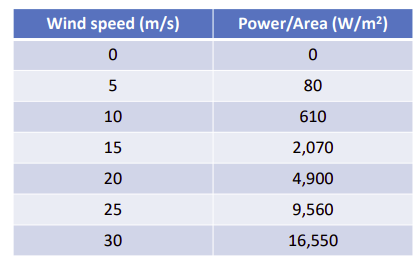
\includegraphics{img/windspeedvpowerinair.png}
\item
  \(C_p\) is the ratio between the actual power obtained and the maximum
  available power.
\item
  The \emph{Betz limit} is the theoretical maximum at 59.3\%.
\end{itemize}

\hypertarget{power-curve}{%
\subsection{Power Curve}\label{power-curve}}

\begin{itemize}
\tightlist
\item
  The speed at which the blades will start to rotate is called the
  \emph{cut in} speed.
\item
  The power output rises with wind speed until it hits a rated power
  output which is the limit of the electrical generator.
\item
  Cut out power involves breaking the system to reduce power.
\end{itemize}

\hypertarget{betz-limit}{%
\subsection{Betz Limit}\label{betz-limit}}

\begin{itemize}
\tightlist
\item
  The simplest model of turbine is actuator disk model.
\item
  The turbine modelled as a circular disc through which air flows with
  velocity \(\vec{v_t}\) with a pressure drop from \(P_1\) to \(P_2\).
\item
  I'm not going to go through derivation yet. Just going to try get some
  exposure to it first.
\item
  One interesting thing, power is \(1/2\cdot{m}v^2\) because
  \(\cdot{m}\) here is the mass flow rate.
\item
  Using mass flow equations to derive what power is for the simple
  actuator model.
\item
  Efficiency can vary with the ratio of upstream (before the turbine)
  and downstream (after the turbine) velocity.
\item
  Can think of it as extracting energy from a specified volume of air
  moving like an object towards the turbine.
\end{itemize}

\begin{center}\rule{0.5\linewidth}{\linethickness}\end{center}

\begin{itemize}
\tightlist
\item
  Turbines do not achieve the Betz limit for several reasons: rotation
  of wake behind rotor, finite number of blades (tip losses), non-zero
  aerodynamic drag.
\item
  The ratio between the speed of the blade tip \(v_{tip}\) and the wind
  speed \(v_0\) is called the tip speed ratio.
\item
  To capture max power tip speed ratio to Cp curve should be kept at a
  maximum.
\end{itemize}

\hypertarget{aerodynamics-of-wind-turbines}{%
\section{Aerodynamics of Wind
Turbines}\label{aerodynamics-of-wind-turbines}}

\begin{itemize}
\tightlist
\item
  More generally, I think this a term represents the dampening factor
  that the turbine has on the air flow through it.
\item
  The mass flow rate of the air is constant. When the rotor disk causes
  this flow velocity to slow it's area after the rotor must increase.
\item
  There's a decrease in Kinetic Energy, a reduction in speed of the mass
  flow of the air. This causes an increase in pressure as the lost of KE
  is transferred to energy in the volume of air.
\item
  There is a drop in this pressure as it passes through the rotor
  disk(?).
\item
  Interesting question: Why not have drag based turbines? So, the rotors
  would be parallel to the wind?
\end{itemize}

\hypertarget{actuator-disk-model}{%
\subsection{Actuator Disk Model}\label{actuator-disk-model}}

\begin{itemize}
\tightlist
\item
  What happens to the kinetic energy that the turbine extracts. It may
  be put to useful work but some of it will be returned to the airflow
  and dissipated as heat.
\item
  It's assumed that the actuator disc (which is just a circular area?)
  induces a velocity variation on the free stream velocity.
\item
  The force on the wind turbine is due to the \textbf{change in
  momentum} of the mass flow.
\item
  \(F = \dot{m}v\)
\end{itemize}

\begin{center}\rule{0.5\linewidth}{\linethickness}\end{center}

\begin{itemize}
\tightlist
\item
  Skipping derivation of force exerted on the air.
\item
  \(F = 2 \rho A_dU_{infty}^2a(1 - a)\)
\item
  Ultimately, the force on the actuator disk is due to the
  \textbf{pressure drop} across it.
\item
  Power is then the rate of work done (\(FU_d\))
\end{itemize}

\hypertarget{rotor-disc-theory}{%
\subsection{Rotor Disc Theory}\label{rotor-disc-theory}}

\begin{itemize}
\item ~
  \hypertarget{due-to-the-rotation-of-the-blades-incoming-air-gains-angular-momentum-a-rotational-component.}{%
  \subsection{Due to the rotation of the blades, incoming air gains
  angular momentum, a rotational
  component.}\label{due-to-the-rotation-of-the-blades-incoming-air-gains-angular-momentum-a-rotational-component.}}
\item
  An \emph{airfoil} is a streamlined shape that is capable of generating
  significantly more lift than drag.
\item
  Lift increases linearly with angle of attack \(\alpha\).
\item
  Drag is more dependent on Reynolds number.
\end{itemize}

\hypertarget{bernoullis-principle-and-continuity}{%
\subsubsection{Bernoulli's Principle and
Continuity}\label{bernoullis-principle-and-continuity}}

\emph{Chapter 14 of Halliday}

\hypertarget{continuity}{%
\paragraph{Continuity}\label{continuity}}

\begin{figure}
\centering
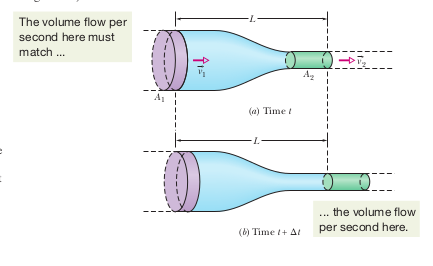
\includegraphics{img/continuityhalliday.png}
\caption{`----'}
\end{figure}

\begin{itemize}
\tightlist
\item
  A \emph{streamline} is a path followed by an individual fluid
  particle.
\item
  A \emph{tube of flow} is a bundle of streamlines.
\item
  The more spacing between streamlines, the lower the pressure, the less
  acceleration imparted by particles on one another.
\item
  Thinking of a garden hose, the velocity of exiting fluid can be
  increased by reducing the area.
\item
  If we consider the fluid incompressible then taking a volume that
  enters on the left side of the tube and equating it with one leaving
  the right side of the tube.
\item
  Volume flows must match at all points in a tube, or all cross
  sections.
\item
  The Volume flow rate: \(\Delta V/\Delta t = Av\) which is a constant.
\item
  If fluid is uniform mass flow rate:
  \(\Delta V/\Delta t \rho = \rho Av\)
\end{itemize}

\hypertarget{bernoullis-principle}{%
\paragraph{Bernoulli's Principle}\label{bernoullis-principle}}

\begin{itemize}
\tightlist
\item
  When the fluid does not change elevation.
\item
  The kinetic energy per unit volume (kinetic energy density).
\item
  If a fluid element increases speed along a horizontal streamline, the
  pressure of the overall fluid must somehow decrease.
\item
  Is this due to the transfer of kinetic energy to this streamline?
\end{itemize}

\hypertarget{assignment-2-notes}{%
\section{Assignment 2 Notes}\label{assignment-2-notes}}

\begin{itemize}
\tightlist
\item
  what is the problem?
\item
  What's the data?
\item
  What's the conditions under which these exist?
\end{itemize}

With the time series data, it's discrete. So binning is used to create a
distribution with probability of a new wind speed measurement falling
within a certain bin.

Why plot with bin edges vs bin centers?

Should I be also looking at wind direction?

\end{document}
